\section{Molecular Mixing Ratios in Thermochemical Equilibrium}

In exoplanetary atmospheres, the abundances of molecules are expected to approach thermochemical equilibrium under high-temperature and high-pressure conditions. Even in cases where vertical transport, photochemistry, or low-temperature atmospheres dominate, it is useful to understand the baseline state under thermochemical equilibrium. Here, we consider how the molecular mixing ratios in the atmosphere are determined when thermochemical equilibrium is established. \\

\subsection*{Conservation of Elements}

In the gas, molecular species such as \ce{H2} and \ce{H2O}, as well as atomic species like \ce{H}, ions, and free electrons, are mixed in appropriate proportions. These are collectively referred to as {\bf species}. In contrast, we also wish to track the total number of atoms contained in all species, e.g., \ce{H}, \ce{O}, \ce{C}, etc. These are referred to as {\bf elements}, distinguished from species. In this text, we denote elements using sans-serif fonts, such as $\Hel$, $\Oel$, and $\Cel$. \\


\subsection*{The Case of a Binary System}

As the simplest example, let us consider a two-species gas composed of hydrogen atoms and molecules:
\begin{align*}
\ce{2 H <--> H2}.
\end{align*}
We ask: what composition ratio is reached at thermochemical equilibrium?\footnote{In reality, a third-body catalyst $M$ makes the process more realistic, as in \ce{2 H + M <--> H2 + M}, but here we ignore $M$ for mathematical clarity.}  
In this case, the species are \ce{H} and \ce{H2} ($N_s = 2$), while the only element is $\Hel$ ($N_e = 1$).

Let us suppose there are $\nel_{\Hel}$ atoms of hydrogen (e.g., 1 mol). The element conservation law is then
\begin{align}
    n_\mathrm{H} + 2 n_\mathrm{H2}  = \nel_{\Hel}.
\end{align}
Given pressure $P$ and temperature $T$, the distribution of $\Hel$ between \ce{H} and \ce{H2} at equilibrium is determined by minimizing the Gibbs free energy. At thermochemical equilibrium, the abundances of species are obtained by
\begin{align}
\label{eq:opt1tce}
    &(n_\mathrm{H}^\ast, n_\mathrm{H2}^\ast) = \mathrm{minimize}_{(n_\mathrm{H}, n_\mathrm{H2})} \,\, G(T, P, n_\mathrm{H}, n_\mathrm{H2}) \,\, \\ 
    &\mbox{subject to} \,\, n_\mathrm{H} + 2 n_\mathrm{H2} =  \nel_{\Hel},  \\
    &G(T, P, n_\mathrm{H}, n_\mathrm{H2}) = n_\mathrm{H} \mu_\mathrm{H} + n_\mathrm{H2} \mu_\mathrm{H2}, \\
     &\, n_\mathrm{H} \ge 0, \, n_\mathrm{H2} \ge 0,
\end{align}
where $\mu_\mathrm{H}$ and $\mu_\mathrm{H2}$ are the chemical potentials of \ce{H} and \ce{H2}. Using the standard-state chemical potentials, these are given by
\begin{align}
    \mu_\mathrm{H} &= \mu_\mathrm{H}^o(T) + RT \log{\frac{P_\mathrm{H}}{P_\mathrm{ref}}} \\
    &=  \mu_\mathrm{H}^o(T) + RT \log{\frac{n_\mathrm{H} P}{(n_\mathrm{H} + n_\mathrm{H2}) P_\mathrm{ref}}}, \\
    \mu_\mathrm{H2} &= \mu_\mathrm{H2}^o(T) + RT \log{\frac{P_\mathrm{H2}}{P_\mathrm{ref}}} \\
    &=  \mu_\mathrm{H2}^o(T) + RT\log{\frac{n_\mathrm{H2} P}{(n_\mathrm{H} + n_\mathrm{H2}) P_\mathrm{ref}}}.
\end{align}
One can verify that $\partial G/\partial n_\mathrm{H} = \mu_\mathrm{H}$ and $\partial G/\partial n_\mathrm{H2} = \mu_\mathrm{H2}$ hold.

To prepare for generalization, let us solve the constrained optimization above using the method of Lagrange multipliers. Define the free parameter vector $\xv = ( n_\mathrm{H},  n_\mathrm{H2}, \lambda )^\top$, then
\begin{align}
\label{eq:opt2tce}
    \xv_\ast &= \mathrm{minimize}_{\xv} \,\, \mathcal{L} (T, P, \xv), \\ 
    \mathcal{L} (T, P, \xv) &\equiv G(T, P, \xv) + \lambda (n_\mathrm{H}  + 2 n_\mathrm{H2} - \nel_{\Hel} ), \\
    \label{eq:nonnegative_tce}
    &n_\mathrm{H} \ge 0, \, n_\mathrm{H2} \ge 0.
\end{align}
The non-negativity conditions will be checked afterward. Setting the derivatives of $\mathcal{L} (T, P, \xv)$ with respect to $\xv$ equal to zero gives
\begin{align}
&\frac{\partial \mathcal{L} (T, P, \xv)}{\partial \xv} = 
\begin{pmatrix}
    \mu_\mathrm{H} + \lambda \\
    \mu_\mathrm{H2} + 2 \lambda \\
    n_\mathrm{H} + 2 n_\mathrm{H2} -  \nel_{\Hel} 
\end{pmatrix} \\
&=
\begin{pmatrix}
    \mu_\mathrm{H}^o(T) + RT \log{\frac{n_\mathrm{H} P}{(n_\mathrm{H} + n_\mathrm{H2}) P_\mathrm{ref}}}  + \lambda \\
    \mu_\mathrm{H2}^o(T) + RT\log{\frac{n_\mathrm{H2} P}{(n_\mathrm{H} + n_\mathrm{H2}) P_\mathrm{ref}}} + 2 \lambda \\
    n_\mathrm{H} + 2 n_\mathrm{H2} -  \nel_{\Hel} 
\end{pmatrix}
=
\begin{pmatrix}
    0 \\
    0 \\
    0
\end{pmatrix}.
\end{align}
Eliminating $\lambda$ from the first two components yields
\begin{align}
    \log{\left( \frac{n_\mathrm{H}^2 }{n_\mathrm{H2} (n_\mathrm{H} + n_\mathrm{H2})} \frac{P}{P_\mathrm{ref}} \right)} =- \frac{2 \mu_\mathrm{H}^o - \mu_\mathrm{H2}^o}{RT}.
\end{align}
Using the third component (the conservation law), $n_\mathrm{H} + 2 n_\mathrm{H2} - \nel_{\Hel}=0$, to eliminate $n_\mathrm{H2}$ gives
\begin{align}
\frac{ \nel_{\Hel}^2 - n_\mathrm{H}^2}{4 n_\mathrm{H}^2} = \frac{P}{P_\mathrm{ref}} 
\exp{\left( - \frac{\mu_\mathrm{H2}^o - 2 \mu_\mathrm{H}^o}{RT} \right)}  \equiv k.
\end{align}
Since $n_\mathrm{H} \ge 0$,
\begin{align}
 \frac{n_\mathrm{H}}{ \nel_{\Hel} } = \frac{1}{\sqrt{4 k + 1}}.
\end{align}
From the conservation law,
\begin{align}
 \frac{n_\mathrm{H2}}{ \nel_{\Hel} } = \frac{1}{2} \left( 1 - \frac{1}{\sqrt{4 k + 1}} \right).
\end{align}
Note that these quantities are expressed per hydrogen element $\nel_{\Hel}$. In practice, one can simply set $\nel_{\Hel} = 1$ mol for calculation.

The volume mixing ratios (VMRs) are then
\begin{align}
 \mathrm{VMR} (\ce{H}) &= \frac{n_\mathrm{H}}{n_\mathrm{tot}} = \frac{1}{2} \left( \sqrt{k^2 + 4 k} - k \right), \\
  \mathrm{VMR} (\ce{H2}) &= \frac{n_\mathrm{H2}}{n_\mathrm{tot}} = \frac{1}{2} \left( 2 + k - \sqrt{k^2 + 4 k}\right).
\end{align}
The temperature dependence of the mixing ratios is shown in Fig.~\ref{fig:temperature_exogibbs}. \\

\begin{figure}
    \centering
    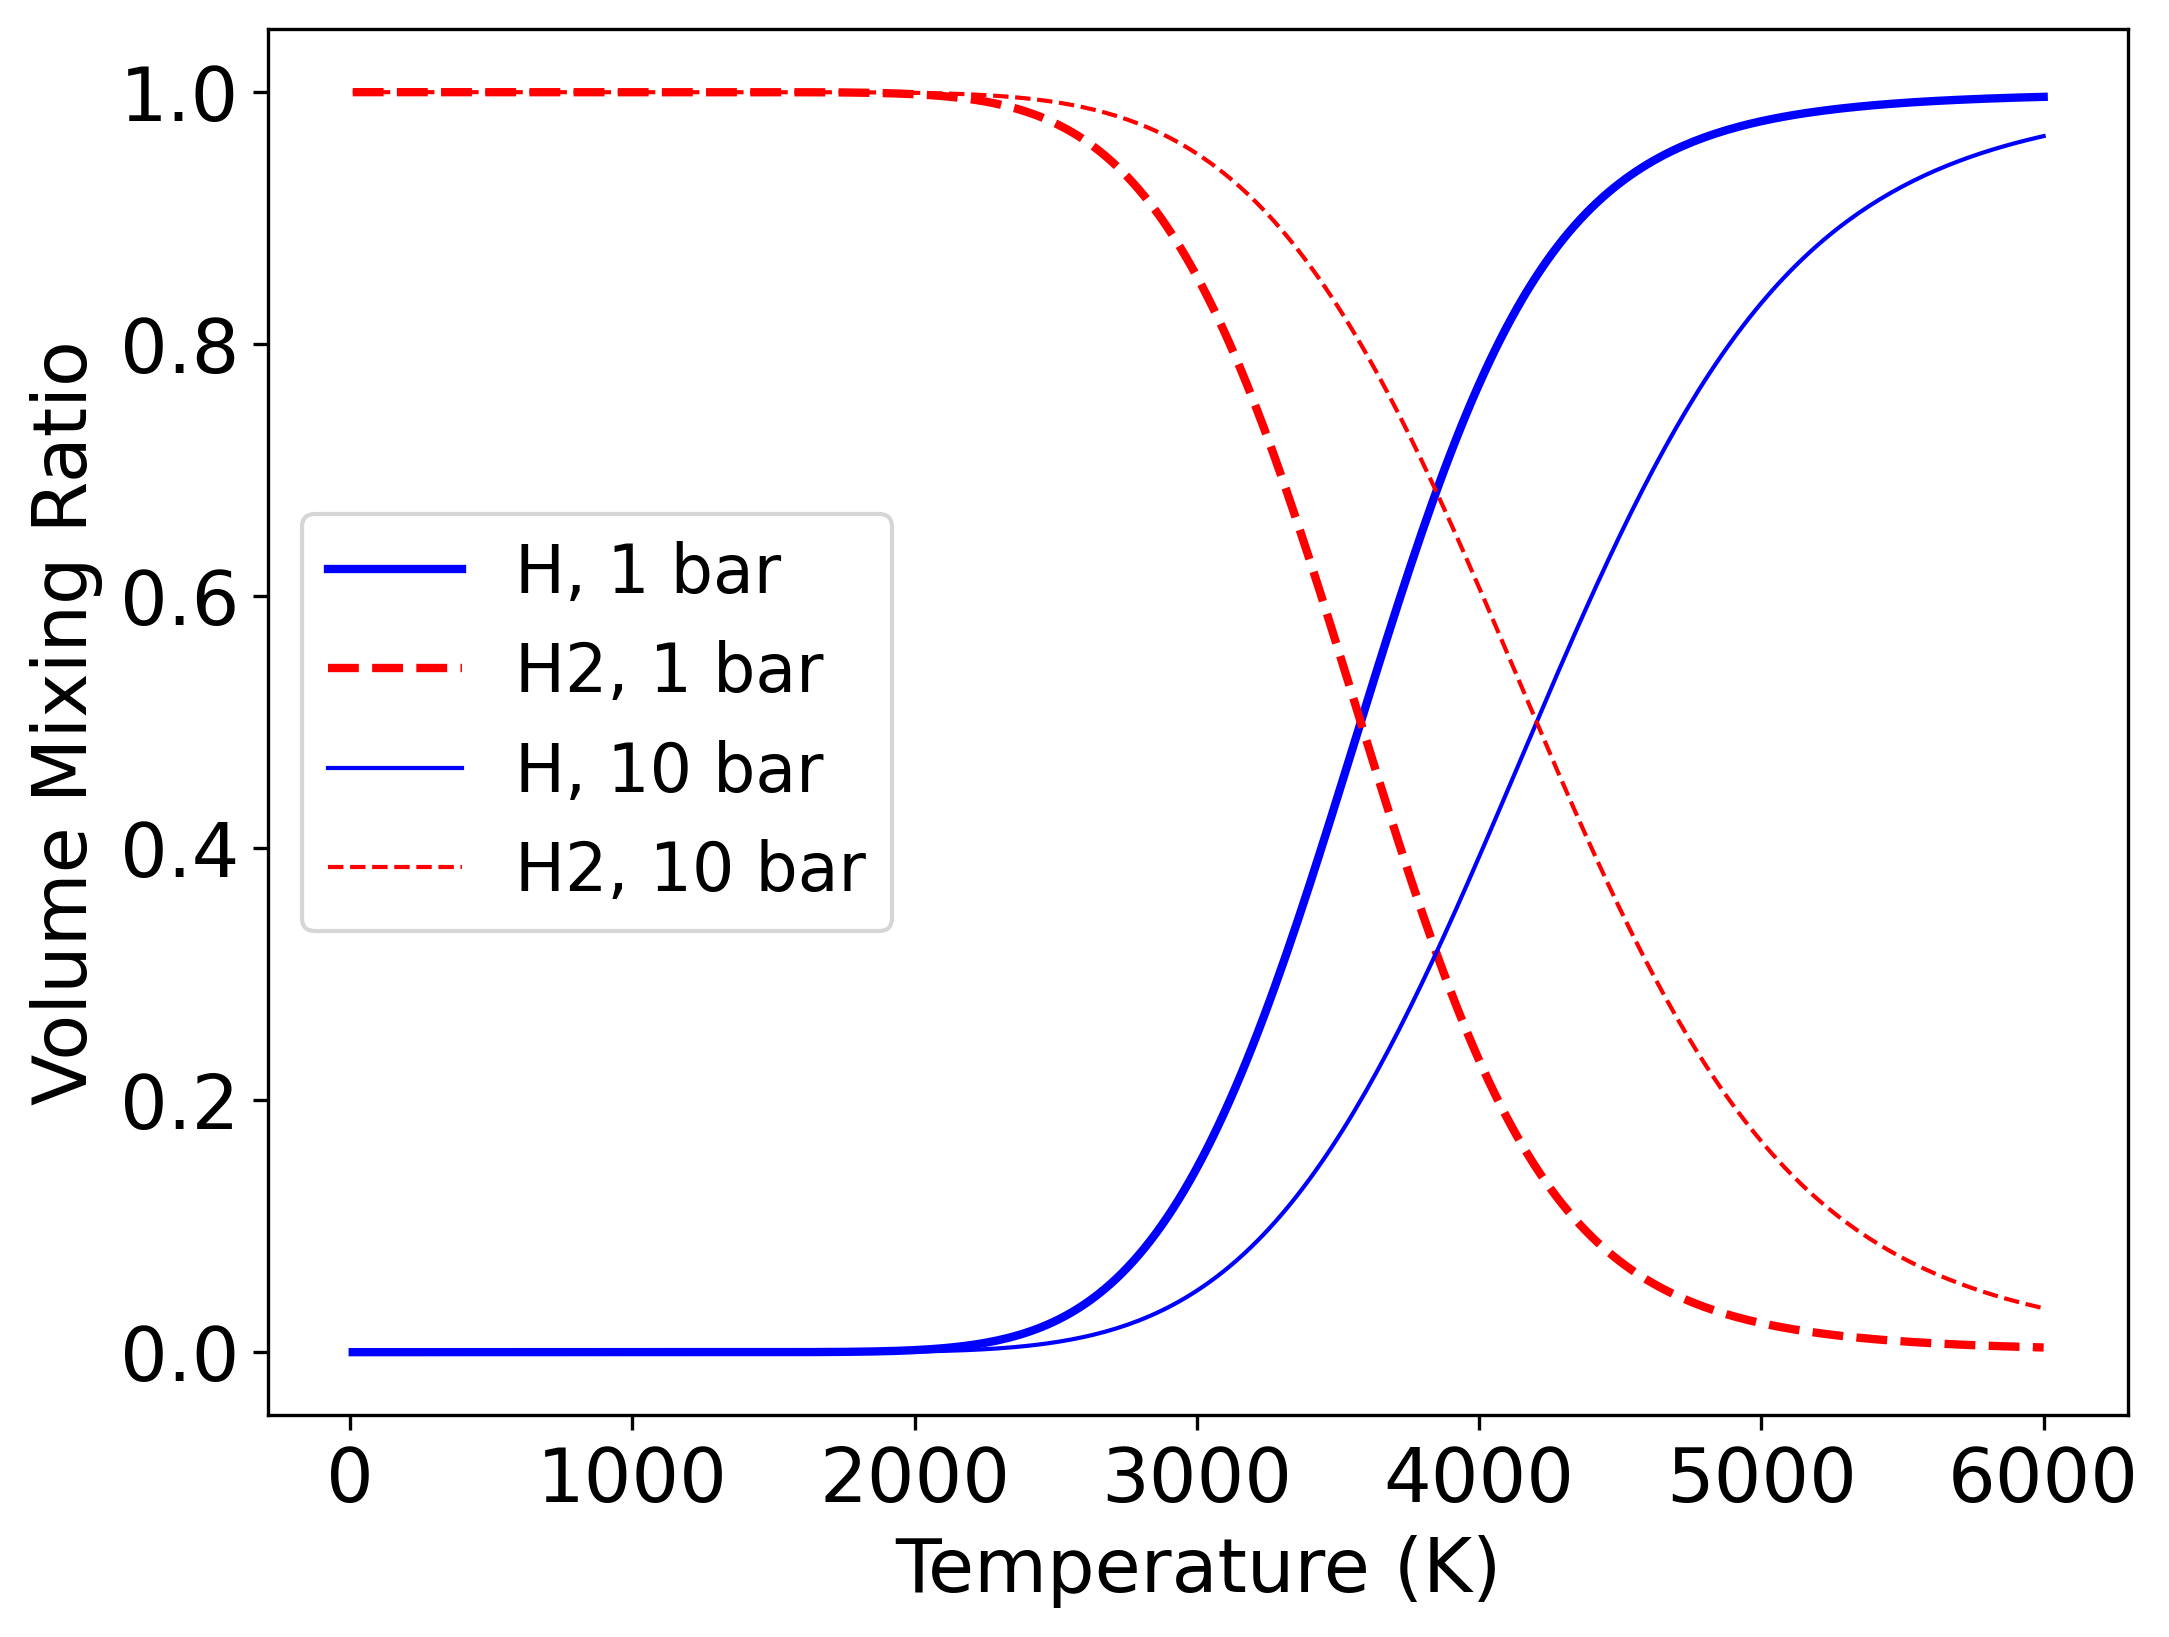
\includegraphics[width=\linewidth]{fig/tce_two_species.png}
    \caption{Volume mixing ratios in thermochemical equilibrium for \ce{2 H <--> H2}.}
    \label{fig:temperature_exogibbs}
\end{figure}

\subsection*{Multi-Component Systems$^\ddagger$}

Next, let us consider a multi-element system.  
As an example, take the elements $\Hel, \Cel, \Oel$, and the species \ce{CO, H2, CH4, H2O}. These constitute the major molecular components in hydrogen-rich atmospheres. The relevant chemical reaction can be written as
\begin{align*}
\ce{CO + 3 H2 <--> CH4 + H2O}.
\end{align*}

In terms of elements, the decomposition of each species is
\begin{align*}
\ce{H2 <--> 2 $\Hel$ \, \, \, \, \, \, \, \, \\
H2O <--> 2 $\Hel$ + 1 $\Oel$ \\
CH4 <--> 4 $\Hel$ + 1 $\Cel$ \\
CO <-->  1 $\Cel$ + 1 $\Oel$},
\end{align*}
or, including zero components explicitly,
\begin{align*}
\ce{H2 <--> 2 $\Hel$ + 0 $\Cel$ + 0 $\Oel$ \\
H2O <--> 2 $\Hel$ + 0 $\Cel$ + 1 $\Oel$ \\
CH4 <--> 4 $\Hel$ + 1 $\Cel$ + 0 $\Oel$ \\
CO <--> 0 $\Hel$ + 1 $\Cel$ + 1 $\Oel$ }.
\end{align*}

From the right-hand sides, we define the formula matrix:
\begin{align*}
  A \equiv
\begin{pmatrix} 
2 & 2 & 4 & 0 \\
0 & 0 & 1 & 1 \\
0 & 1 & 0 & 1 
\end{pmatrix}.
\end{align*}

Let the vector of species abundances be $\nv = (n_\mathrm{H_2}, n_\mathrm{H_2 O},n_\mathrm{CH_4},n_\mathrm{CO})^\top$, and the vector of elemental abundances be $\bv = (\nel_\Hel, \nel_\Cel, \nel_\Oel)^\top$ (note the distinction between elemental abundances and species). Then the elemental conservation law is expressed as
\begin{align}
    A \, \nv = \bv.
\end{align}

For a multi-element system, the equilibrium abundances are obtained by minimizing the Gibbs free energy:
\begin{align}
\label{eq:gibss_multi}
    \nv^\ast &= \mathrm{minimize}_{\nv} G(T, p, \nv) \nonumber \\
    &\mbox{subject to} \,\, A \, \nv = \bv, \, n_i \ge 0, \\
    G(T, p, \nv) &\equiv  \muv (T, P, \nv)^\top \nv, \\ 
    \label{eq:chemical_potential_mu}
    \muv (T, p, \nv) &=  \muv^\circ(T) + RT \log{\left(\frac{p}{\ntot} \nv\right)} ,
\end{align}
where the total number density and normalized pressure are defined as
\begin{align}
\label{eq:ntot_tce}
    \ntot &= \sum_i n_i, \\
    p &\equiv P/P_\mathrm{ref}.
\end{align}

For the \ce{CO, H2, CH4, H2O} system, Eq.~(\ref{eq:gibss_multi}) becomes
\begin{align}
    \mathcal{L}(T, p, \nv,\lambdav) &= \sum_{i = \ce{CO, H2, CH4, H2O}} \mu_i (T) \, n_i \nonumber \\ 
    &+ \lambda_{\Hel} (2 n_{\ce{H2}} + 4 n_{\ce{CH4}} + 2 n_{\ce{H2O}} - b_\Hel) \nonumber \\
    &+ \lambda_{\Cel} (n_{\ce{CO}} + n_{\ce{CH4}} - b_\Cel) \nonumber \\ 
    &+ \lambda_{\Oel} (n_{\ce{CO}} + n_{\ce{H2O}} - b_\Oel).
\end{align}

Here we follow the implementation of NASA/CEA (Chemical Equilibrium with Applications) by Gordon and McBride \cite{gordon1994computer,2024arXiv241207166G}. In CEA, minimization of the Gibbs free energy is carried out using a quadratic Lagrange multiplier method. That is,
\begin{align}
    (\nv^\ast, \lambdav)  &= \mathrm{minimize}_{(\nv,\lambdav)} \,\, \mathcal{L}(T, p, \nv, \lambdav), \\
    \mathcal{L}(T, p, \nv,\lambdav) &= G(T, p, \nv) + \lambdav^\top \left(A \nv - \bv\right),
\end{align}
where at this stage the non-negativity condition $n_i \ge 0$ is not yet enforced.

To find stationary points of $\mathcal{L}(T, p, \nv, \lambdav)$, we define, with the optimization variables $\yv = (\nv, \lambdav)$,
\begin{align}
\label{eq:fv_tea0}
    \fv(\yv) &\equiv \frac{\partial}{\partial \yv} \mathcal{L}(T, p, \yv).
\end{align}
The solution is obtained by solving
\begin{align}
    \label{eq:fv_tea}
    \fv(\yv^\ast) = \boldsymbol{0}
\end{align}
using Newton’s method, yielding $\yv^\ast = (\nv^\ast, \lambdav^\ast)$.  

Next, computing the $\nv$-component of Eq.~(\ref{eq:fv_tea0}) gives
\begin{align}
\label{eq:Lpartialn}
    \frac{\partial}{\partial \nv}   \mathcal{L}(T, p, \nv, \lambdav) =  \muv (T, P, \nv) + A^\top \lambdav,
\end{align}
where we have used the thermodynamic identity $\partial_{\nv} G(T, p, \nv) =  \muv (T, P, \nv)$\footnote{This can be verified directly from Eq.~(\ref{eq:chemical_potential_mu}).} together with $\lambdav^\top (A \nv) = (A^\top \lambdav)^\top \nv$ and $\partial_{\xv} (S^\top \xv) = S$.  
Note that Eq.~(\ref{eq:Lpartialn}) is linear in $\lambdav$.  

The $\lambdav$-component simply enforces the conservation relations:
\begin{align}
\label{eq:Lpartiall}
\frac{\partial}{\partial \lambdav}  \mathcal{L}(T, p, \nv, \lambdav) = A \nv - \bv.
\end{align}

Using Eq.~(\ref{eq:chemical_potential_mu}), the system of equations to be solved by Newton’s method in Eq.~(\ref{eq:fv_tea}) is
\begin{align}
\label{eq:Lpartialnx}
    \frac{\muv^\circ(T)}{RT}+ \log{\left(\frac{p}{\ntot^\ast} \nv^\ast \right)} + \frac{A^\top \lambdav^\ast}{RT}   &= \boldsymbol{0}, \\
    A \nv^\ast - \bv &= \boldsymbol{0},
\end{align}
where $\ntot^\ast$ is a function of $\nv^\ast$:
\begin{align}
\ntot^\ast &= \sum_i n_i^\ast.
\end{align}



Here, the CEA algorithm employs several tricks. First, to solve Eq.~(\ref{eq:fv_tea}), we add $\ntot$ as an independent variable. Since $\ntot$ originally depended on $\nv$ via Eq.~(\ref{eq:ntot_tce}), we include this relation—namely Eq.~(\ref{eq:ntot_tce})—as a constraint (rather than as a prerequisite). Furthermore, we reparameterize $\nv$ and $\ntot$ by taking logarithms, i.e., we adopt $\lnnv = \ln{\nv}$ and $\lnntot = \ln{\ntot}$ as independent variables. This transformation naturally enforces the non-negativity constraints $n_i \ge 0$, and, by working in log-space, yields numerically stable computations over a wide dynamic range. 

With these changes, we introduce the new variable set $\zv = (\lnnv, \lambdav, \lnntot)$, and the system to be solved is
\begin{align}
\label{eq:Lpartialncea}
    \Fv_n (\zv) &\equiv \frac{\muv^\circ(T)}{RT} + \lnnv - \lnntot \, \uv + \log{p} \, \uv  + \frac{A^\top \lambdav}{RT},  \\
    \Fv_\lambda (\zv) &\equiv A e^{\lnnv} - \bv = \boldsymbol{0}_M, \\
    F_\mathrm{tot} (\zv) &\equiv \sum_i {e^{q_i}} - e^{\lnntot} = 0,
\end{align}
whose solution satisfies
\begin{align}
  \Fv_n (\zv) &= \boldsymbol{0}_M, \\
  \Fv_\lambda (\zv) &= \boldsymbol{0}_M, \\
  F_\mathrm{tot} (\zv) &= 0.
\end{align}
Here $\boldsymbol{0}_M$ denotes the $M$-dimensional zero vector. The solution is $\zv^\ast = (\lnnv^\ast, \lambdav^\ast, \lnntot^\ast)$. For brevity we sometimes write $\Fv (\zv) = (\Fv_n (\zv), \Fv_\lambda (\zv), F_\mathrm{tot} (\zv))$.

Newton’s method requires the Jacobian $\Jv (\zv) = \partial \Fv / \partial \zv$:
\begin{align}
\label{eq:jacobian_tce}
\Jv (\zv) &=
\left(
\begin{array}{ccc}
    \dfrac{\partial \Fv_n}{\partial \lnnv}  & \dfrac{\partial \Fv_n}{\partial \lambdav}& \dfrac{\partial \Fv_n}{\partial \lnntot}\\ 
    \dfrac{\partial \Fv_\lambda}{\partial \lnnv} & \dfrac{\partial \Fv_\lambda}{\partial \lambdav} & \dfrac{\partial \Fv_\lambda}{\partial \lnntot} \\
    \dfrac{\partial F_\mathrm{tot}}{\partial \lnnv} & \dfrac{\partial F_\mathrm{tot}}{\partial \lambdav} & \dfrac{\partial F_\mathrm{tot}}{\partial \lnntot} \\  
\end{array}
\right) \nonumber \\
&=
\left(
\begin{array}{ccc}
 E_M &  \dfrac{A^\top}{RT} & - \uv\\ 
 Y(\lnnv) & Z_M & \boldsymbol{0}_M \\ 
 (e^{\qv})^\top & \boldsymbol{0}_M^\top & - e^\lnntot\\  
\end{array}
\right),
\end{align}
where $E_M$ is the $M \times M$ identity matrix, $Z_M$ is the $M \times M$ zero matrix, and $M$ is the number of elements (the length of $\bv$). The matrix $Y(\lnnv)$ is defined by
\[
Y(\lnnv)= A \, \mathrm{diag}(e^{\lnnv}),
\]
i.e., with components
\begin{align}
Y_{ij} = A_{ij} e^{q_j}.
\end{align}

From Eq.~(\ref{eq:second_newton}), the Newton update satisfies $\Jv (\zv_k) \, \Delta \zv = - \Fv (\zv_k)$, i.e.,
\begin{align}
    \left(
\begin{array}{ccc}
 E_M &  \dfrac{A^\top}{RT} & - \uv\\ 
 Y(\lnnv) & Z_M & \boldsymbol{0}_M \\ 
 (e^{{\lnnv}_k})^\top & \boldsymbol{0}_M^\top & - e^{(\lnntot)_k}\\  
\end{array}
\right)
    &\left(
\begin{array}{c}
\Delta \lnnv \\
\Delta \lambdav \\
\Delta \lnntot
\end{array}
\right) \nonumber \\
= -
    &\left(
\begin{array}{c}
\Fv_n (\zv_k) \\
\Fv_\lambda(\zv_k) \\
F_\mathrm{tot} (\zv_k)
\end{array}
\right).
\end{align}
Thus the update $\Delta \zv = (\Delta \lnnv, \Delta \lambdav, \Delta \lnntot)$ satisfies
\begin{align}
\label{eq:update_tce_1_}
    &\Delta \lnnv + \frac{A^\top \Delta \lambdav}{RT} - \Delta \lnntot \, \uv \nonumber \\
    &= -\frac{\muv^\circ(T)}{RT} - {\lnnv}_k + (\lnntot)_k \, \uv - \log{p} \, \uv  - \frac{A^\top \lambdav_k}{RT}, \\
\label{eq:update_tce_2_}
    &Y(\lnnv_k) \Delta \lnnv = A \left(e^{\lnnv_k} \odot \Delta \lnnv\right) = \bv - A e^{\lnnv_k}, \\
\label{eq:update_tce_3_}
    &(e^{\lnnv_k})^\top \Delta \lnnv  - e^{(\lnntot)_k} \Delta \lnntot = e^{(\lnntot)_k} - \sum_i {e^{(q_i)_k}} .
\end{align}

Only Eq.~(\ref{eq:update_tce_1_}) involves $\Delta \lambdav$ and $\lambdav_k$. Since we are not directly interested in $\lambdav$, we introduce a new update variable
\begin{align}
    \piv \equiv - \frac{\Delta \lambdav + \lambdav}{RT},
\end{align}
and update $\lnnv, \piv, \lnntot$ instead. (Because $\piv$ is a throwaway variable, we omit $\Delta$ on it.) Then Eq.~(\ref{eq:update_tce_1_}) becomes
\begin{align}
\label{eq:update_tce_1x}
    \Delta \lnnv &=  A^\top \piv + \Delta \lnntot \, \uv - \gv_k(T), \\
    \gv_k (T) &\equiv \frac{\muv^\circ(T)}{RT} + {\lnnv}_k - (\lnntot)_k \, \uv + \log{p} \, \uv .
\end{align}
Hence, once $\piv$ and $\Delta \lnntot$ are determined, we can compute the desired $\Delta \lnnv$. Substituting Eq.~(\ref{eq:update_tce_1x}) into Eqs.~(\ref{eq:update_tce_2_}) and (\ref{eq:update_tce_3_}) yields the following system of $M+1$ linear equations:
\begin{align}
    &A \, \mathrm{diag} (e^{\lnnv_k}) \, A^\top \, \piv + \Delta \lnntot \, A e^{\lnnv_k} \nonumber \\
    &= A \left(e^{\lnnv_k} \odot \gv_k (T) \right) + \bv - A  e^{\lnnv_k}, \\
    &(A  e^{\lnnv_k})^\top \piv + \Delta \lnntot \, \left( \sum_i e^{(\lnnv_k)_i} - e^{(\lnntot)_k} \right) \nonumber \\ 
    &= (e^{\lnnv_k})^\top \gv_k(T) + e^{(\lnntot)_k} - \sum_i {e^{(q_i)_k}} .
\end{align}
In the above, we retained $\lnnv_k$ and $(\lnntot)_k$ explicitly, but in code it is often clearer to revert $e^{\lnnv}$ to $\nv$. Define
\begin{align}
    B &\equiv  A \, \mathrm{diag} (\nv_k) \, A^\top, \\
    \bv_k &\equiv A \nv_k, \\
    \delta \bv_k &\equiv \bv - \bv_k, \\
     \delta n_\mathrm{tot,k} &\equiv  \sum_i n_{k,i} - (n_\mathrm{tot})_{k},
\end{align}
where $n_{k,i}$ denotes the $i$-th component of $\nv_k$. Then we obtain
\begin{align}
\label{eq:rgie1}
   B \, \piv + \Delta \lnntot \, \bv_k &= A \left( \nv_k \odot \gv_k (T) \right) + \delta \bv_k, \\
\label{eq:rgie2}
\bv_k \cdot \piv + \delta n_\mathrm{tot, k} \, \Delta \lnntot &= \nv_k \cdot \gv_k(T) - \delta n_\mathrm{tot,k}.
\end{align}
This linear system in $\piv$ and $\Delta \lnntot$ is referred to as the \emph{Reduced Gibbs Iteration Equations}.
